In weighted Jacobi, the preconditioning matrix is given by $\mathbf{M}^{-1} = \omega \left( \diag {\color{burgundy}\mathbf{A}} \right)^{-1}$, where $\omega$ is the weighting factor.
Following the derivation from Section \ref{sec:lfahighorder}, the symbol of the weighted Jacobi error propagation operator is therefore given by
\begin{equation}
\tilde{\mathbf{S}} \left( \omega, \boldsymbol{\theta} \right) = I - \tilde{\mathbf{M}}^{-1} \left( \omega, \boldsymbol{\theta} \right) \tilde{{\color{burgundy}\mathbf{A}}} \left( \boldsymbol{\theta} \right) = I - \omega \left( \mathbf{Q}^T \left( \diag {\color{burgundy}\mathbf{A}}^e \right)^{-1} \mathbf{Q} \right) \tilde{{\color{burgundy}\mathbf{A}}} \left( \boldsymbol{\theta} \right),
\end{equation}
where this expression has been simplified by the fact that $e^{\imath \left( x_i - x_i \right) \theta / h} = 1$.

\begin{definition}
The symbol of the error propagation operator for weighted Jacobi smoothing is given by
\begin{equation}
\tilde{\mathbf{S}} \left( \nu, \omega, \boldsymbol{\theta} \right) = \left( I - \omega \left( \mathbf{Q}^T \left( \diag {\color{burgundy}\mathbf{A}}^e \right) \mathbf{Q} \right)^{-1} \tilde{{\color{burgundy}\mathbf{A}}} \left( \boldsymbol{\theta} \right) \right)^\nu,
\end{equation}
where $\nu$ is the number of smoothing passes and $\omega$ is the weighting parameter.
\label{def:jacobi_symbol}
\end{definition}

\begin{figure}[!ht]
  \centering
  \subfloat[Spectrum of 1D Jacobi for $p = 4$]{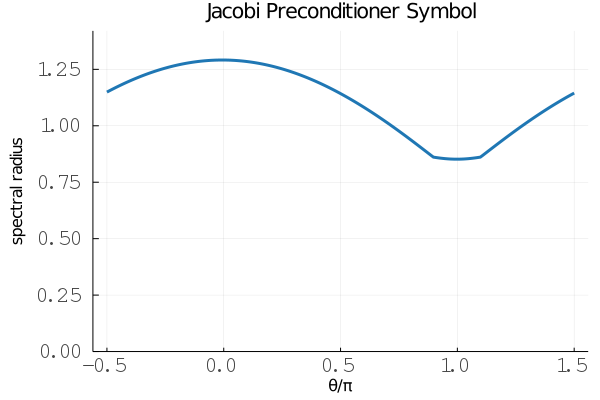
\includegraphics[width=0.48\textwidth]{../img/JacobiSymbol1D}\label{fig:jacobi_spectrum_1d}}
  \hfill
  \subfloat[Spectrum of 2D Jacobi for $p = 4$]{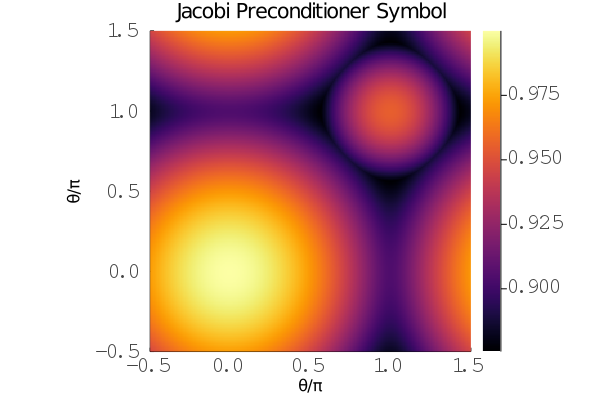
\includegraphics[width=0.48\textwidth]{../img/JacobiSymbol2D}\label{fig:jacobi_spectrum_2d}}
  \caption{Spectrum of Jacobi Preconditioner Symbol}
\end{figure}

Using Definition \ref{def:jacobi_symbol}, in Figures \ref{fig:jacobi_spectrum_1d} and \ref{fig:jacobi_spectrum_2d}, we see the spectral radius of the symbol of unweighted Jacobi preconditioning for the scalar diffusion operator with a fourth-order H1 Lagrange finite element basis on the Gauss-Lobatto points in one and two dimensions.
In Figure \ref{fig:jacobi_spectrum_1d}, we see that the unweighted Jacobi still has a spectral radius greater than $1.0$; this spectral radius can be improved by changing the weighting factor, $\omega$.

\begin{figure}[!ht]
  \centering
  \subfloat[Spectral Radius of Weighted Jacobi for $p = 4$]{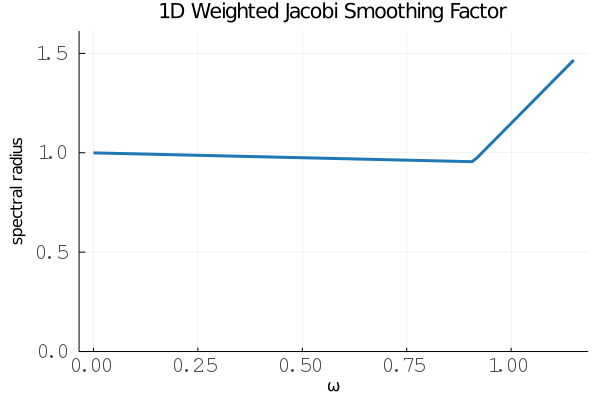
\includegraphics[width=0.48\textwidth]{../img/weightedJacobiSymbol1D}\label{fig:weighted_jacobi_radius_1d}}
  \hfill
  \subfloat[Spectral Radius of Weighted Jacobi for $p = 4$]{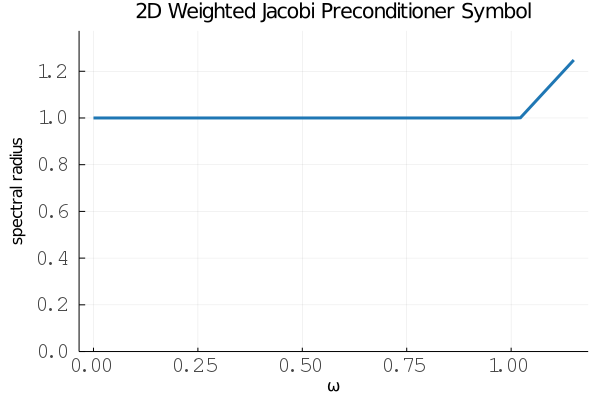
\includegraphics[width=0.48\textwidth]{../img/weightedJacobiSymbol2D}\label{fig:weighted_jacobi_radius_2d}}
  \caption{Spectral Radius of Weighted Jacobi Preconditioner Symbol}
\end{figure}

In Figures \ref{fig:weighted_jacobi_radius_1d} and \ref{fig:weighted_jacobi_radius_2d}, we see the spectral radius of the symbol of weighted Jacobi preconditioning for the scalar diffusion operator with a fourth-order H1 Lagrange finite element basis on the Gauss-Lobatto points in one and two dimensions as a function of the weighting parameter, $\omega$.
In one dimension, the optimal smoothing parameter is approximately $\omega \approx 0.86$, while in two dimensions the optimal smoothing parameter is approximately $\omega \approx 1.0$.
Both figures indicate that underestimating the optimal smoothing parameter has a relatively mild effect compared to the increase in the spectral radius of the symbol from overestimating the optimal smoothing parameter.

As discussed in \cite{he2020two}, the classical optimal smoothing parameter is given by
\begin{equation}
\omega = \frac{2}{\lambda_{\text{min}, H} + \lambda_{\text{max}, H}}
\end{equation}
for weighted Jacobi, where $H$ indicates the high frequency range.
Unfortunately, as noted by \cite{he2020two}, this optimal smoothing parameter does not result in optimal two-grid convergence.
He and MacLachlan observed this discrepancy for h-multigrid on uniformly spaced nodes, but we will also observe this discrepancy for p-multigrid.
